

\tikzset{every picture/.style={line width=0.75pt}} %set default line width to 0.75pt        

\begin{tikzpicture}[x=0.75pt,y=0.75pt,yscale=-1,xscale=1]
%uncomment if require: \path (0,374); %set diagram left start at 0, and has height of 374

%Image [id:dp7152221511204973] 
\draw (269.48,152.73) node  {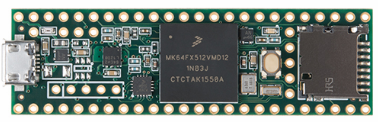
\includegraphics[width=197.45pt,height=60.59pt]{Figures/TikzFigures/layOut/teensy.PNG}};
%Image [id:dp37486105933332636] 
\draw (366.16,279.14) node [rotate=-180.22,xslant=-0.01] {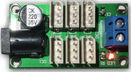
\includegraphics[width=89.36pt,height=69.95pt]{Figures/TikzFigures/layOut/supl.PNG}};
%Image [id:dp9034481830242995] 
\draw (132.79,272.76) node [rotate=-359.65,xslant=0] {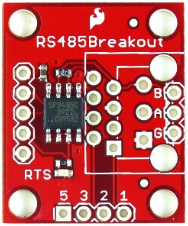
\includegraphics[width=83.35pt,height=72.71pt]{Figures/TikzFigures/layOut/rs.PNG}};
%Image [id:dp11028803786694708] 
\draw (236.5,45.39) node [rotate=-270] {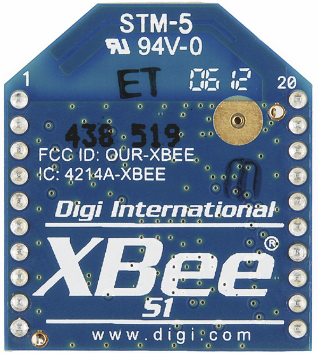
\includegraphics[width=60.59pt,height=62.4pt]{Figures/TikzFigures/layOut/bee.PNG}};
%Left Arrow [id:dp5012443384308891] 
\draw   (438.55,274.06) -- (457.33,256.75) -- (457.33,265.41) -- (485.5,265.41) -- (485.5,282.72) -- (457.33,282.72) -- (457.33,291.38) -- cycle ;
%Right Arrow [id:dp0023557246216043826] 
\draw   (80.2,146.67) -- (111.93,146.67) -- (111.93,137.72) -- (133.09,155.61) -- (111.93,173.5) -- (111.93,164.56) -- (80.2,164.56) -- cycle ;
%Straight Lines [id:da08227247794525927] 
\draw [color={rgb, 255:red, 247; green, 10; blue, 10 }  ,draw opacity=1 ][line width=1.5]    (150.92,81.17) -- (150.52,123.87) ;


%Straight Lines [id:da025924835708441174] 
\draw [color={rgb, 255:red, 247; green, 10; blue, 10 }  ,draw opacity=1 ][line width=1.5]    (217.48,81.17) -- (150.92,81.17) ;


%Straight Lines [id:da00602413999639384] 
\draw [color={rgb, 255:red, 247; green, 10; blue, 10 }  ,draw opacity=1 ][line width=1.5]    (42.76,80.79) -- (155.28,80.79) ;


%Straight Lines [id:da7149252935730617] 
\draw [color={rgb, 255:red, 247; green, 10; blue, 10 }  ,draw opacity=1 ][line width=1.5]    (43.55,80.79) -- (43.55,256.21) ;


%Straight Lines [id:da3829700368795059] 
\draw [color={rgb, 255:red, 247; green, 10; blue, 10 }  ,draw opacity=1 ][line width=1.5]    (91.09,256.21) -- (43.55,256.21) ;


%Straight Lines [id:da8981864779638247] 
\draw [line width=1.5]    (31.67,88.48) -- (31.67,290.84) ;


%Straight Lines [id:da6466608797084847] 
\draw [line width=1.5]    (91.89,290.07) -- (31.67,290.07) ;


%Straight Lines [id:da35185368144106244] 
\draw [line width=1.5]    (31.67,88.48) -- (272.55,89.25) ;


%Straight Lines [id:da8387196090383506] 
\draw    (271.76,80.02) -- (271.76,89.25) ;


%Straight Lines [id:da36845317589148996] 
\draw [color={rgb, 255:red, 91; green, 235; blue, 46 }  ,draw opacity=1 ][line width=1.5]    (225.01,81.56) -- (160.03,184.66) ;


%Straight Lines [id:da4171143722401429] 
\draw [color={rgb, 255:red, 248; green, 231; blue, 28 }  ,draw opacity=1 ][line width=1.5]    (231.55,81.56) -- (173.71,184.66) ;


%Straight Lines [id:da33656991606038633] 
\draw [color={rgb, 255:red, 32; green, 240; blue, 26 }  ,draw opacity=1 ][line width=1.5]    (90.3,273.91) -- (208.5,229) -- (256.5,185) ;


%Straight Lines [id:da3740974102672152] 
\draw [color={rgb, 255:red, 244; green, 250; blue, 27 }  ,draw opacity=1 ][line width=1.5]    (266.5,186) -- (215.5,236) -- (90.5,266) ;


%Straight Lines [id:da18281067478913027] 
\draw [color={rgb, 255:red, 24; green, 81; blue, 146 }  ,draw opacity=1 ][line width=1.5]    (91.09,282.37) -- (220.5,243) -- (275.5,185) ;


%Straight Lines [id:da7137403407481466] 
\draw [line width=1.5]    (180.34,279.84) -- (343.47,319.08) ;


%Straight Lines [id:da9319303523938192] 
\draw [color={rgb, 255:red, 243; green, 20; blue, 20 }  ,draw opacity=1 ][line width=1.5]    (180.34,271.18) -- (344.5,305) ;


%Straight Lines [id:da7229658725423573] 
\draw [color={rgb, 255:red, 74; green, 144; blue, 226 }  ,draw opacity=1 ][line width=1.5]    (180.34,262.52) -- (343.5,296) ;


%Straight Lines [id:da43545523008986176] 
\draw [line width=1.5]    (31.5,202) -- (150.5,202) ;


%Straight Lines [id:da5107595655280059] 
\draw [line width=1.5]    (150.5,183) -- (150.5,202) ;



% Text Node
\draw (99.41,156.19) node  [align=left] {USB};
% Text Node
\draw (465.49,273.68) node  [align=left] {12V};
% Text Node
\draw (77,191) node  [align=left] {Gnd};
% Text Node
\draw (98,71) node  [align=left] {5V};
% Text Node
\draw (257,310) node  [align=left] {Gnd};
% Text Node
\draw (263,265) node  [align=left] {Rs 485};
% Text Node
\draw (338,106) node  [align=left] {Teensy 3.5};
% Text Node
\draw (320,30) node  [align=left] {Xbee receiver};
\draw (133,341) node  [align=left] { \ \ \ BOB-10124\\Rs 285 toRs 485};
\draw (338,341) node  [align=left] {Supply board\\for dynamixel servo's };
% Text Node
\draw (219,101) node  [align=left] {Tx1 \ \ \ Rx1};
% Text Node
\draw (200,212) node  [align=left] {RxTx2};
% Text Node
\draw (333,212) node  [align=left] {Transmit enable wire};


\end{tikzpicture}